% Maerz 2015
% Autor: Mandy Vogel
% Tests 
\documentclass[xcolor={table}]{beamer}
\usetheme{Singapore}

%% \usepackage{listings}
\usepackage{linkimage}

\begin{document}

\title{Numeric Data}   
\author{Mandy Vogel} 
\date{\today}
%\logo{\includegraphics[scale=0.14]{PIC1}}

\begin{frame}
\titlepage
\end{frame}

\begin{frame}
\frametitle{Table of Contents}\tableofcontents
\end{frame}


\section{Numeric Summaries}
\begin{frame}\frametitle{Numeric summaries}
  To describe data we need a proper way to summarize them for easier understanding. Therefore we focus on three main areas:
  \begin{itemize}
  \item parameters of location (today)
  \item spread (today) and
  \item shape (later)
  \end{itemize}
\end{frame}


\begin{frame}\frametitle{Exercises} 
  \begin{enumerate}
  \item load the data \textit{ZA5240\_v2-0-0.sav} from the data directory using the \texttt{spss.get()} function from the Hmisc package (data source: gesis.org, General Social Survey 2014), assign the data set to a variable with a appropriate name.
  \item the file \textit{variablenliste.txt} contains a list with the variable description (only available in German)
  \item how many rows? (\texttt{nrow()})
  \item how many columns? (\texttt{ncol()})
  \end{enumerate}
\end{frame}


\subsection{Location Parameters}
\begin{frame}\frametitle{Location parameters}
  \begin{itemize}
  \item a location parameter is a central or typical value for a distribution
  \item typical location parameters are:
    \begin{itemize}
    \item mean (\texttt{mean()})
    \item trimmed means (\texttt{mean()})
    \item median (\texttt{median()})
    \item mode 
    \end{itemize}
  \end{itemize}  
\end{frame}

\begin{frame}[allowframebreaks]\frametitle{Mean and median}
How to interpret the mean?
  \begin{itemize}
  \item graphically, it is the visual balance point of the given values (physics formula for the center of mass)
  \item this demonstrates a weakness of the mean when used to represent \textit{center}
  \item the \textit{trimmed mean} tries to make the mean more stable by trimming from both sides a certain percentage of the most extreme values
  \item if mean and the trimmed mean are substantially different the data are very likely to be skewed
  \item the trimmed mean pushed to its limits (by trimming 50\% of the data from each end) leaves us with basically a single value: the median
  \item so the median is the value which divides the values into the 50\% lowest and the 50\% highest values
  \end{itemize}  
\end{frame}

\begin{frame}\frametitle{Exercises} 
  \begin{enumerate}
  \item the column V417 contains the net income, calculate the mean using the \texttt{mean()} function! What is the problem?
  \item again calculate the mean but now the trimmed version (using the \texttt{trim=T} argument). What is the conclusion?
  \end{enumerate}
\end{frame}


\begin{frame}\frametitle{Other measures of position}
  \begin{itemize}
  \item the concept of the median can be generalized: as the median splits the data in half (with half the data smaller and the other half larger), the $p$th quantile is basically the value in the data set for which $100\cdot p$  is less than the value and $100 \cdot (1-p)$ is more (so the median is the 0.5 quantile); special cases of quantiles are percentiles, quartiles and quintiles (\texttt{quantiles()})
  \item hinges (not often mentioned but used in boxplots; \texttt{fivenum()})
  \item and of course min and max (\texttt{min(), max()})
  \end{itemize}  
\end{frame}

\begin{frame}[fragile]\frametitle{Exercises} 
  \begin{enumerate}
  \item summarize the net income using \texttt{summary(), quantile()} and \texttt{fivenum}!
  \item make a boxplot by using the following syntax! (we also use column V81 - gender and V86 - graduation)
\begin{verbatim}
  require(ggplot2)
  ggplot(x, aes(x=V86, y=V417)) +
      geom_boxplot()  
\end{verbatim}
\item add gender as coloring
\begin{verbatim}
  ggplot(x, aes(x=V86, y=V417, fill=V81)) +
      geom_boxplot()
\end{verbatim}
  \end{enumerate}
\end{frame}


\begin{frame}\frametitle{So what now?}
  \begin{itemize}
  \item so we se - there is a difference in income between male and female people
  \item the next step would be to test if this difference is statistically significant, but therefore we need also the measure of spread (even if you do not use it explicitly in testing) so there are
  \end{itemize}
\end{frame}

\subsection{Parameters of Spread}
\begin{frame}[allowframebreaks]\frametitle{Spread}
  \begin{itemize}
  \item these are parameters which measure the variability in the data
  \item there is e.g. the range (\texttt{range()})
  \item the sample variance (\texttt{var()}) and
  \item the sample standard deviation (\texttt{sd()}) which is simply the square root of the variance
  \item the coefficient of variation which is the standard deviation normalized by the mean
  \item the IQR (interquartile range; \texttt{IQR} - there are nine ways to calculate it - so different statistics software can have different IQRs - depending on the method)
  \item the mad (median absolute deviation)
  \end{itemize}
\end{frame}

\section{Hypothesis Testing}
\begin{frame}\frametitle{four possible situations}\footnotesize
\begin{tabular}{cl|c|c|}
  &  \multicolumn{1}{c}{}& \multicolumn{2}{c}{\textbf{Situation}} \\
  &  \multicolumn{1}{c}{}& \multicolumn{1}{c}{$H_0$ is true} & \multicolumn{1}{c}{$H_0$ is false} \\
\cline{3-4}
\textbf{Conclusion} & $H_0$ is not rejected &  Correct decision  & Type II error \\
\cline{3-4}
 & $H_0$ is rejected & Type I error &  Correct decision  \\
\cline{3-4}
\end{tabular}
\end{frame}


\subsection{Common symbols}
\begin{frame}\frametitle{Common symbols}
  \rowcolors[]{1}{gray!10}{gray!30}
  \begin{tabular}{@{} >{\ttfamily}l l@{}} 
    \rowcolor{gray!40}symbol & meaning \onslide<2->\\
    $n$ & number of observations (sample size)\onslide<2->\\
    $K$ & number of samples (each having $n$ elements) \onslide<3->\\
    $\alpha$ & level of significance \onslide<3->\\
    $\nu$ & degrees of freedom \onslide<3->\\
    $\sigma$ & standard deviation (population)\onslide<3->\\
    $s$ & standard deviation (sample)\onslide<4->\\
    $\mu$ & population mean \onslide<4->\\
    $\bar{x}$ & sample mean \onslide<4->\\
    $\rho $ & population correlation coefficient \onslide<4->\\
    $r$ & sample correlation coefficient \onslide<5->\\
    $Z$ & standard normal deviate \\
  \end{tabular}
\end{frame}

\begin{frame}\frametitle{Alternatives}
    \only<1>{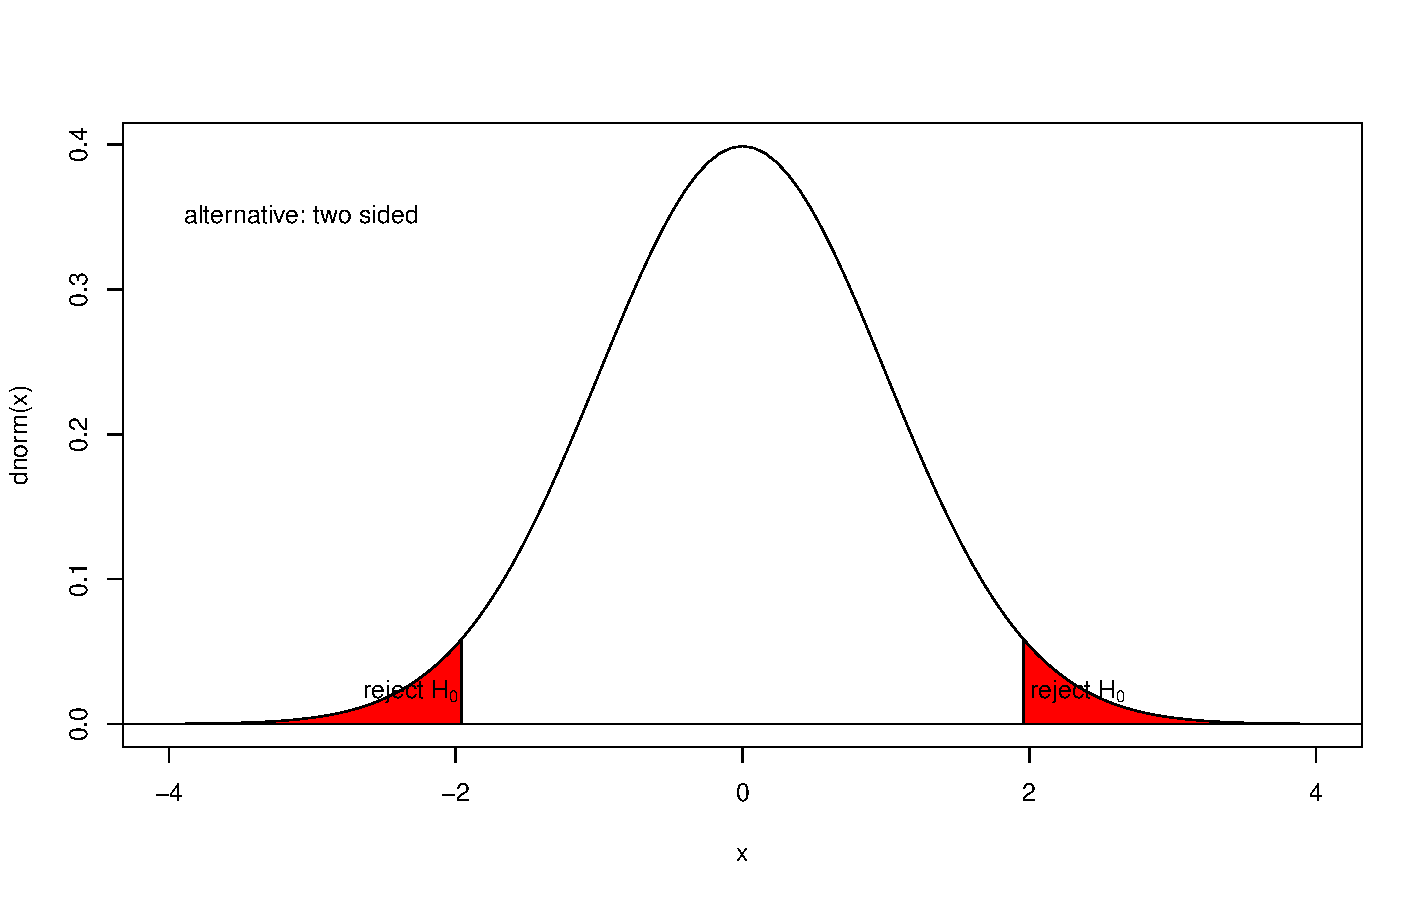
\includegraphics[width=11cm, height=7cm]{twosided.pdf}}
    \only<2>{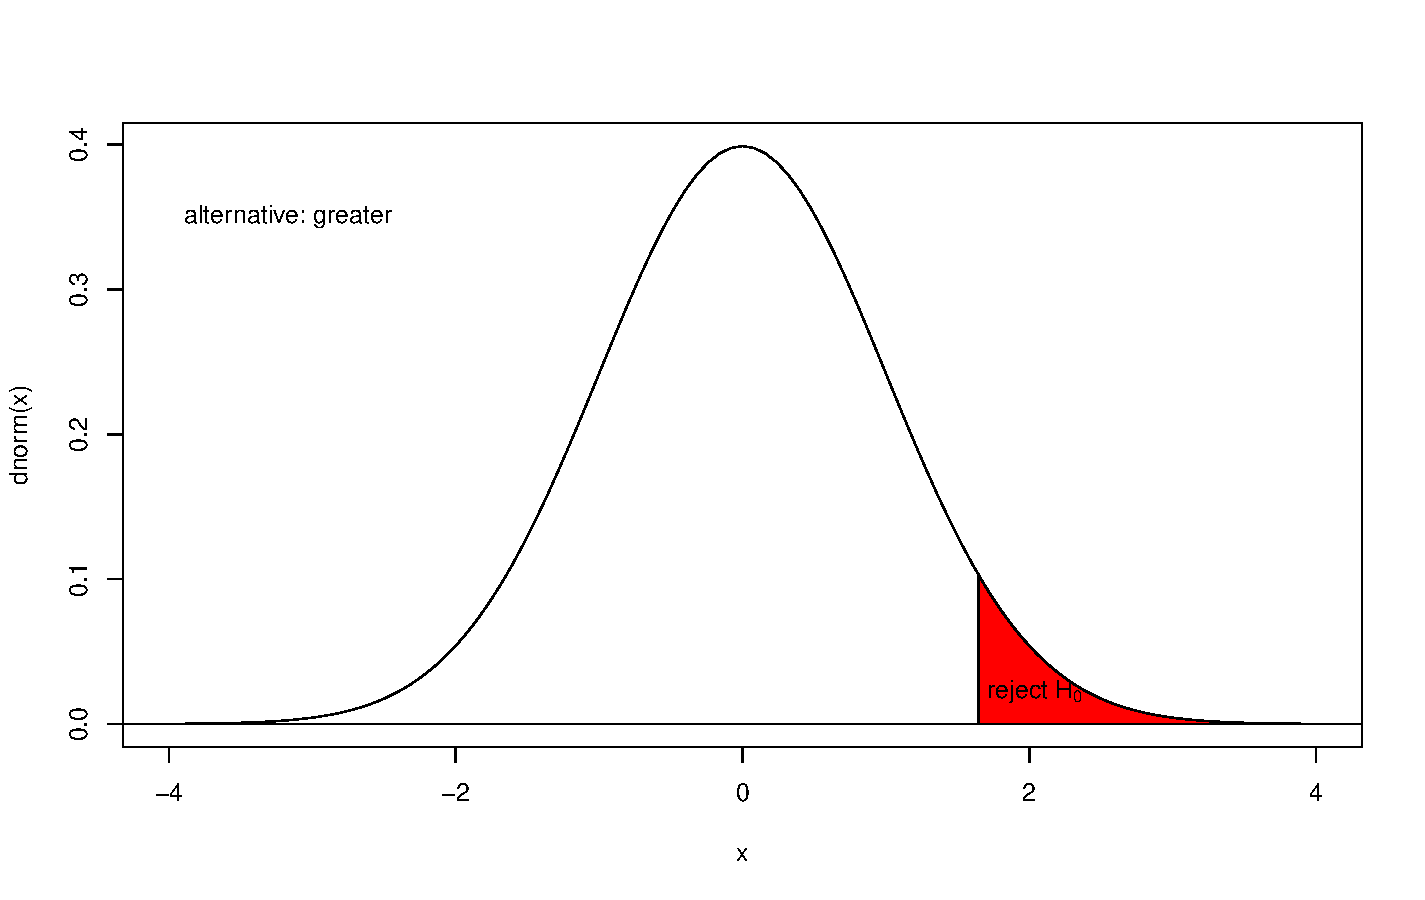
\includegraphics[width=11cm, height=7cm]{greater.pdf}}
    \only<3>{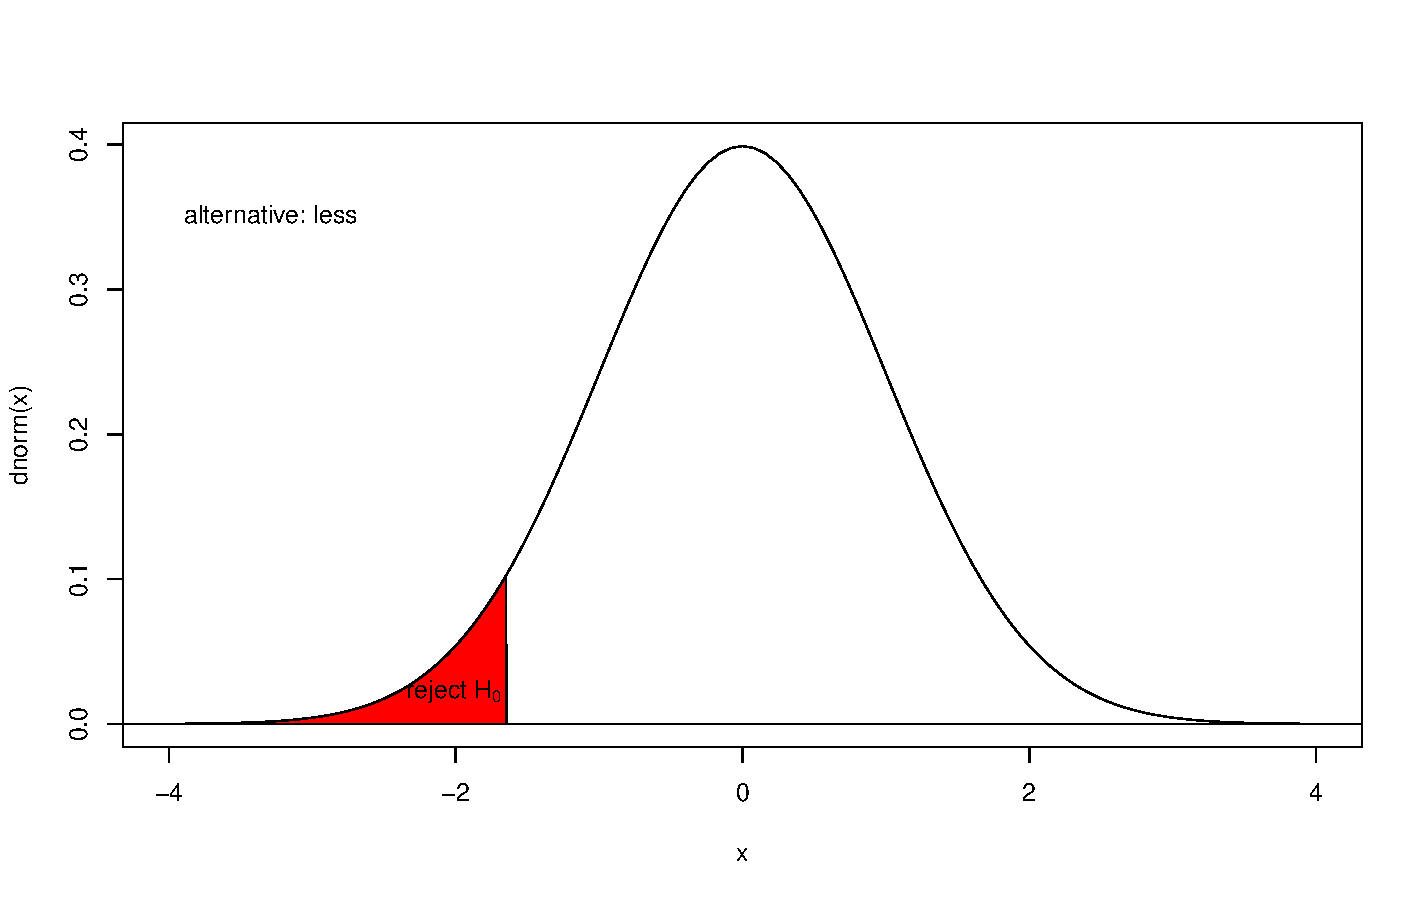
\includegraphics[width=11cm, height=7cm]{less.pdf}}
\end{frame}


\begin{frame}\frametitle{p-value}
  \begin{alertblock}{Note:}
    The p-value is the probability of the sample estimate (of the respective estimator) under the null. We do not know anything of probabilities of the null or of estimates under the alternative!
  \end{alertblock}
\end{frame}

\section{T Test}

\begin{frame}\frametitle{William Gosset}
  \begin{itemize}
  \item the t-test is called t-test because its test statistic is t distributed (this distribution was discovered or invented or whatsoever by William Gosset)
  \item so we take our data 
  \item calculate some mystic t-value
  \item compare this value with the distribution of t-values under the null
  \item and then we decide: is our t value so unlikely, that we can reject the null (wow! lower than 5\% - is 5\% really that low...??? - this cutoff level was suggested by Fisher in the 1920s, so it is not a part of the decalogue and - therefore - there is no guarantee linked to it)
  \end{itemize}
\end{frame}


\begin{frame}\frametitle{t-test}
There is not only one t-test, there is 
  \begin{itemize}
  \item the one sample t-test
  \item the two sample t-test assuming equal variances
  \item the two sample t-test without the former assumption
  \item the paired t-test (in fact: this is a one sample t-test against 0)
  \end{itemize}
But: there is only one command in R: \texttt{t.test()}
\end{frame}

\subsection{One Sample t-test}

\defverbatim{\ttesta}{
\begin{verbatim}
> set.seed(1)
> x <- rnorm(12)
> t.test(x,mu=0) ## population mean 0

	One Sample t-test

data:  x
t = 1.1478, df = 11, p-value = 0.2754
alternative hypothesis: true mean is not equal to 0
95 percent confidence interval:
 -0.2464740  0.7837494
sample estimates:
mean of x 
0.2686377 
\end{verbatim}
}


\defverbatim{\ttestb}{
\begin{verbatim}


> t.test(x,mu=1) ## population mean 1

	One Sample t-test

data:  x
t = -3.125, df = 11, p-value = 0.009664
alternative hypothesis: true mean is not equal to 1
95 percent confidence interval:
 -0.2464740  0.7837494
sample estimates:
mean of x 
0.2686377 
\end{verbatim}
}

\begin{frame}[fragile]\frametitle{t-tests}
\begin{itemize}
\item \emph{one sample t-test}: test a sample mean against a population mean
$$ t = \frac{\bar{x}-\mu_0}{s/\sqrt{n}}$$ where $\bar{x}$ is the sample mean, $s$ is the sample standard deviation and $n$ is the sample size. The degrees of freedom used in this test is $n-1$
\end{itemize}
\end{frame}

\begin{frame}[fragile]\frametitle{One Sample t-test}
\only<1>{\ttesta}
\only<2>{\ttestb}
\end{frame}


\subsection{Two Sample t-tests}


\begin{frame}[fragile]\frametitle{Two Sample t-tests}
There are two ways to perform a two sample t-test in R:
\begin{itemize}
\item given two vectors \texttt{x} and \texttt{y} containing the measurement values from the respective groups \texttt{t.test(x,y)}
\item given one vector \texttt{x} containing all the measurement values and one vector \texttt{g} containing the group membership $t.test(x \sim g)$ (read: x dependend on g)
\end{itemize}
\end{frame}

\begin{frame}[fragile]\frametitle{Two Sample t-tests: two vector syntax}\footnotesize
\begin{verbatim}
> set.seed(1)
> x <- rnorm(12)
> y <- rnorm(12)
> g <- sample(c("A","B"),12,replace = T)
> t.test(x,y)

	Welch Two Sample t-test

data:  x and y
t = 0.5939, df = 20.012, p-value = 0.5592
alternative hypothesis: true difference in means is not equal to 0
95 percent confidence interval:
 -0.5966988  1.0717822
sample estimates:
 mean of x  mean of y 
0.26863768 0.03109602   
\end{verbatim}
\end{frame}


\begin{frame}[fragile]\frametitle{Two Sample t-tests: formula syntax}\footnotesize
\begin{verbatim}




> t.test(x ~ g)

	Welch Two Sample t-test

data:  x by g
t = -0.6644, df = 6.352, p-value = 0.5298
alternative hypothesis: true difference in means is not equal to 0
95 percent confidence interval:
 -1.6136329  0.9171702
sample estimates:
mean in group A mean in group B 
      0.1235413       0.4717726 
\end{verbatim}
\end{frame}


\begin{frame}[fragile]\frametitle{Welch/Satterthwaite vs. Student}
  \begin{itemize}
  \item if not stated otherwise \texttt{t.test()} will not assume that the variances in the both groups are equal
  \item if one knows that both populations have the same variance set the \texttt{var.equal} argument to TRUE to perform a student's t-test
  \end{itemize}
\end{frame}

\begin{frame}[fragile]\frametitle{Student's t-test}\footnotesize
\begin{verbatim}



> t.test(x, y, var.equal = T)

	Two Sample t-test

data:  x and y
t = 0.5939, df = 22, p-value = 0.5586
alternative hypothesis: true difference in means is not equal to 0
95 percent confidence interval:
 -0.5918964  1.0669797
sample estimates:
 mean of x  mean of y 
0.26863768 0.03109602   
\end{verbatim}
\end{frame}

\begin{frame}[fragile]\frametitle{t-test}
  \begin{itemize}
  \item the t-test, especially the Welch test is appropriate whenever the values are normally distributed
  \item it is also recommended for group sizes $\geq 30$ (robust against deviation from normality)
  \end{itemize}
\end{frame}

\begin{frame}\frametitle{Exercises} 
  \begin{enumerate}
  \item do a t-test of income (V417): male against female (V81)!
  \item and compare the bmi (V279) in smokers and non-smokers (V272) and between people with high and normal blood pressure (V242)
  \item how would you interpret the results?
  \item make the appropriate plots!
  \end{enumerate}
\end{frame}


\end{document}
